\documentclass{report}
% Comment the following line to NOT allow the usage of umlauts
\usepackage[utf8]{inputenc}
% Uncomment the following line to allow the usage of graphics (.png, .jpg)
%\usepackage{graphicx}
\usepackage{geometry}
\geometry{left=4cm,right=4cm,top=3cm,bottom=3cm}
\usepackage[all]{xy}
\usepackage{tikz}
\usepackage{amsmath,amsfonts,amssymb,ntheorem}
\usepackage{bigints}
\usepackage[shortlabels]{enumitem}
\usepackage{mleftright}

\newcommand\expt[1]{\mathrm{E}\mleft[\hspace{1pt}#1\hspace{1pt}\mright]}
\newcommand\coex[2]{\mathrm{E}\mleft[\hspace{1pt}#1\,\middle|\, #2\hspace{1pt}\mright]}

\theorembodyfont{\upshape}					
\newtheorem{definition}{Definition}[section]
\newtheorem{example}{Example}[section]
\newtheorem{theorem}{Theorem}[section]
\newtheorem{proposition}{Proposition}[section]
\newtheorem{lemma}{Lemma}[section]
\theoremstyle{nonumberplain}
\theoremheaderfont{\itshape}
\theorembodyfont{\normalfont}
\theoremsymbol{\\\rightline{$\square$}}
\newtheorem{proof}{Proof.}
% Start the document
\begin{document}
\begin{center}
	\textsc{\Huge Measure Theory and}
	~\\
	\vspace{1em}  
	\textsc{\Huge Probability Theory}	
\end{center}
\vspace{1em} 
\tableofcontents
% Create a new 1st level heading
\chapter{Measures}
\section{Class of sets}
If $2^\Omega$ denotes the power set of the set $\Omega$ and a collection of subsets $\mathcal{C}\subset2^\Omega$, we say $\mathcal{C}$ is defined on $\Omega$.

For convenience, let's define some operations on a collection of sets $\mathcal{C}\in 2^{\Omega}$.
\begin{itemize}
	\item Given $f:\Sigma\to\Omega$, $f^{-1}(\mathcal{C}):=\{f^{-1}(A)\in\Sigma\mid A\in\mathcal{C}\}$,
	\item Given $B\subset \Omega$, $B\cap \mathcal{C}:=\{B\cap A\mid A\in\mathcal{C}\}$.
\end{itemize}
\begin{definition}[semiring]
	A nonempty family of sets $\mathcal{S}$ is called a \emph{semiring (of sets)} if the following three statements are true for all sets $A$ and $B$,
	\begin{enumerate}[(1)]
		\item $\varnothing\in \mathcal{S}$
		\item $A,B\in \mathcal{S}$ implies $A\cap B\in\mathcal{S}$ 
		\item $A,B\in \mathcal{S}$ implies $A-B=\cup_{i=1}^n C_i$, where $\{C_{i}\}_{i=1}^{n}$ is a collection of pairwise disjoint sets in $\mathcal{S}$.
	\end{enumerate}	
	Since condition (3) together with $\mathcal{S} \neq \varnothing$ implies that $\varnothing \in \mathcal{S}$, conditions (1) is actually unnecessary.
\end{definition}

\begin{definition}[ring]
	A nonempty family of sets $\mathcal{R}$ is called a \emph{ring (of sets)} if it is closed under finite union and difference. That is, the following two statements are true for all sets $A$ and $B$,
	\begin{enumerate}[(1)]
	\item $A,B\in \mathcal{R}$ implies $A\cup B\in\mathcal{R}$ 
	\item $A,B\in \mathcal{R}$ implies $A-B\in\mathcal{R}$.
	\end{enumerate}	
\end{definition}

A ring of sets $\mathcal{R}$ is a ring in the context of abstract algebra with the operations intersection(multiplication) and symmetric difference(addition), where the multiplicative identity is the set $\cup_{A\in \mathcal{R}} A$. 

\begin{definition}[semialgebra\textsuperscript{\#1}]
	A subring $\mathcal{S}$ defined on $\Omega$ is called an \emph{semialgebra} if it contains $\Omega$. 
\end{definition}

\begin{definition}[semialgebra\textsuperscript{\#2}]
	A collection of sets $\mathcal{S}\subset 2^{\Omega}$ is called an  \emph{semialgebra} the following two statements are true for all sets $A$ and $B$,
	\begin{enumerate}[(1)]
		\item $A,B\in \mathcal{S}$ implies $A\cap B\in\mathcal{S}$ 
		\item $A\in \mathcal{S}$ implies $A^c=\cup_{i=1}^n C_i$, where $\{C_{i}\}_{i=1}^{n}$ is a collection of pairwise disjoint sets in $\mathcal{S}$.
	\end{enumerate}	
\end{definition}

\begin{example}
	\[
	\mathcal{C} \equiv\{(a, b]\in\mathbb{R}\mid-\infty \leq a \leq b<\infty\} \cup\{(a, \infty)\in\mathbb{R}\mid-\infty \leq a<\infty\}
	\]
	is a semialgebra on $\mathbb{R}$.
\end{example}

\begin{definition}[algebra\textsuperscript{\#1}]
	A ring $\mathcal{F}$ defined on $\Omega$ is called an \emph{algebra (of sets)} if it contains $\Omega$. 
\end{definition}

\begin{proposition}
	Every ring is a semiring.
\end{proposition}
\begin{proof}
	Let $\mathcal{R}$ be a ring. First we see $\varnothing=A-A\in \mathcal{R}$. Second, it is straightforward to check
	$$A\cap B=(A\cup B-(A-B))-(B-A)\in\mathcal{R}.$$
	Finally, it is a trivial fact that $A-B=C_1\in\mathcal{R}$. Thus we show the ring $\mathcal{R}$ is also a semiring.
\end{proof}
The following equivalent definitions of algebra are common to see.
\begin{definition}[algebra\textsuperscript{\#2}]
	A collection of sets $\mathcal{F}\subset 2^{\Omega}$ is called an  \emph{algebra (of sets)} if
	\begin{enumerate}
		\item [(a)] $\Omega\in\mathcal{F}$, 
		\item [(b)] $A \in\mathcal{F}$ implies $A^c\in\mathcal{F}$, 
		\item [(c)] $A,B\in\mathcal{F}$ implies $A\cup B\in\mathcal{F}$.
	\end{enumerate}
\end{definition}
An algebra of sets is an associative algebra over a field in the context of abstract algebra: it is a ring and also a vector space over the field $F_2$ of 2 elements, which makes it an $F_2$-algebra. 

\begin{proposition}
	Every algebra is a ring.
\end{proposition}
\begin{proof}
	Note it holds that 
	\[
	A-B=A\cap B^c=(A^c\cup B)^c.
	\]
\end{proof}

\begin{example}
	Let $\Omega$ be a nonempty set, and let $\#A$ denote the number of elements of a set $A\subset\Omega$. Then
	\[
	\mathcal{F} = \{A\subset \Omega : \text{ either }\#A\text{ is finite or }\#A^c\text{ is finite}\}
	\]
	is an algebra defined on $\Omega$.
\end{example}

\begin{definition}[$\sigma$-algebra]
A class $\mathcal{F}\subset 2^{\Omega}$ is called a \emph{$\sigma$-algebra} if it is an algebra and if it satisfies
\begin{enumerate}
	\item [(d)] $A_n\in\mathcal{F}$ for $n\ge 1$ $\implies$ $\bigcup\limits_{n=1}^\infty A_n\in\mathcal{F}$.
\end{enumerate}
\end{definition}
Under the assumption that $\mathcal{F}$ is an algebra, condition (d) can be replaced by a weaker condition (d'), which leads to the following equivalent definition.

\begin{definition}[$\sigma$-algebra]
	A class $\mathcal{F}\subset 2^{\Omega}$ is called a \emph{$\sigma$-algebra} if it is an algebra and if it satisfies
	\begin{enumerate}
		\item [(d')] $A_n\in\mathcal{F},\ A_n\subset A_{n+1}$ for $n\ge 1$ $\implies$ $\bigcup\limits_{n=1}^\infty A_n\in\mathcal{F}$.
	\end{enumerate}
\end{definition}

\begin{example}
	Let $\Omega$ be a nonempty set. Then
	\[
	\mathcal{F} = \{A\subset \Omega : \text{ either }A\text{ is a countable set or }A^c\text{ is a countable set}\}
	\]
	is a $\sigma$-algebra defined on $\Omega$.
\end{example}
It is easy to check the intersection of a family of $\sigma$-algebras on $\Omega$ is also a $\sigma$-algebra. However, the union of two $\sigma$-algebras may not even be an algebra. In many instances, given an arbitrary collection of subsets of $\Omega$, one would like to extend it to a $\sigma$-algebra by adding extra subsets of $\Omega$ as few as possible. This leads to the following definition.

\begin{definition}[$\sigma$-algebra generated by sets]
If $\mathcal{A}\subset2^\Omega$, then the \emph{$\sigma$-algebra generated by} $\mathcal{A}$, denoted by $\sigma(\mathcal{A})$, is defined as
\[
\sigma(\mathcal{A})=\bigcap_{\mathcal{F}\in\mathcal{I}(\mathcal{A})}\mathcal{F}
\]
where $\mathcal{I}(\mathcal{A})=\{\mathcal{F}:\mathcal{A}\subset \mathcal{F}\text{ and }\mathcal{F}\text{ is a }\sigma\text{-algebra defined on }\Omega\}$ is the collection of all $\sigma$-algebras containing the class $\mathcal{A}$.
\end{definition}
Note that since the power set $2^\Omega$ contains $\mathcal{A}$ and is itself a $\sigma$-algebra defined on $\Omega$, the collection $\mathcal{I}(\mathcal{A})$ is not empty and hence, the intersection in the above definition is well defined.

\begin{definition}[Borel $\sigma$-algebra]
	The \emph{Borel $\sigma$-algebra} on a topological space $\mathbb{S}$ is defined as the $\sigma$-algebra	generated by the collection of open sets in $\mathbb{S}$.
\end{definition}


\begin{example}
	Let $\mathcal{B}(\mathbb{R}^k)$ denote the Borel $\sigma$-algebra on the Euclidean space $\mathbb{R}^k$ with standard topology, $1\le k < +\infty$. Then, $\mathcal{B}(\mathbb{R}^k)=\sigma(\{A : A\text{ is an open subset of } \mathbb{R}^k\})$
	is also generated by each of the following classes of sets
	\begin{align*}
	\mathcal{O}_1&=\{(a_1, b_1)\times\cdots\times(a_k,b_k):-\infty\le a_i< b_i\le+\infty,1\le i\le k\};\\
	\mathcal{O}_2&=\{(-\infty, x_1)\times\cdots\times(-\infty,x_k):x_i\in\mathbb{R},1\le i\le k\};\\
	\mathcal{O}_3&=\{(a_1, b_1)\times\cdots\times(a_k,b_k):a_i, b_i\in\mathbb{Q},a_i<b_i,1\le i\le k\};\\
	\mathcal{O}_4&=\{(-\infty, x_1)\times\cdots\times(-\infty,x_k):x_i\in\mathbb{Q},1\le i\le k\}.\\
	\end{align*}
\end{example}

\begin{definition}[$\pi$-system]
	A class $\mathcal{C}$ of subsets of $\Omega$ is a $\pi$-system or a $\pi$-class if 
	\[
	A,B\in\mathcal{C} \implies A\cap B \in \mathcal{C}.
	\]
\end{definition}
\begin{example}
	The classes $\mathcal{O}_i\ (i=1,2,3,4)$ in Example 1.1.3 are all $\pi$-systems.
\end{example}
\begin{definition}[$\lambda$-system]
A class $\mathcal{L}$ of subsets of $\Omega$ is a $\lambda$-system or a $\lambda$-class if
\begin{enumerate}
	\item [(a)] $\Omega\in \mathcal{L}$,
	\item [(b)] $A,B\in\mathcal{L},A \subset B\implies B\setminus A\in\mathcal{L}$,
	\item [(c)] $A_n \in\mathcal{L},A_n\subset A_{n+1}$ for all $n\ge1$ $\implies A_n\in\mathcal{L}$ for $n\ge1$.
\end{enumerate}
\end{definition}

\begin{example}
	Every $\sigma$-algebra is a $\lambda$-system.
\end{example}

\begin{theorem}
	If $\mathcal{C}$ is a $\pi$-system, then $\lambda(\mathcal{C})=\sigma(\mathcal{C})$.
\end{theorem}



\section{Measurable Space}
\begin{definition}[measurable space]
	Given a nonempty set $\Omega$ and a $\sigma$-algebra $\mathcal{F}$ on  $\Omega$, the tuple $(\Omega,\mathcal{F})$ is called a \emph{measurable space}.
\end{definition}

\begin{definition}[measurable map]
	Given two measurable spaces $(\Omega,\mathcal{F})$ and $(S,\mathcal{S})$, the map $f:\Omega\to S$ is $\mathcal{F}/\mathcal{S}$-\emph{measurable} if
	\[
	f^{-1}(B)\in\mathcal{F},\quad\forall B\in\mathcal{S} .
	\]
	We say $f$ is measurable if the underlying $\sigma$-algebras $\mathcal{F}$ and $\mathcal{S}$ are self-evident. 
\end{definition}
Note $f^{-1}$ preserves $\sigma$-algebra, which leads to the following definition.

\begin{definition}[$\sigma$-algebra generated by measurable map]
	Assume $f$ is a measurable map from $(\Omega,\mathcal{F})$ to $(S,\mathcal{S})$. The $\sigma$-algebra generated by $f$ is defined as
	\[
	\sigma(f):=\sigma\left(f^{-1}(\mathcal{S})\right)=f^{-1}(\mathcal{S}).
	\]
\end{definition}
$\sigma(f)$ is the smallest $\sigma$-algebra on $\Omega$ such that $f$ is $\mathcal{F}/\mathcal{S}$-\emph{measurable}. That is,  
\[
	\text{$f$ is $\mathcal{F}/\mathcal{S}$-\emph{measurable}}\implies \sigma(f)\subset\mathcal{F}.
\] 

\begin{definition}[tensor product $\sigma$-algebra ]
	Let $(\Omega_1,\mathcal{F}_1)$ and $(\Omega_2,\mathcal{F}_2)$ be two measurable spaces. Denote by $\mathcal{F}_1\otimes\mathcal{F}_2$ the $\sigma$-algebra on the Cartesian product $\Omega_1\times\Omega_2$ generated by subsets of the form $B_1\times B_2$, where $B_{1}\in\mathcal{F}_1$ and $B_{2}\in\mathcal{F}_2$, i.e., 
	\[
	\mathcal{F}_{1} \otimes \mathcal{F}_{2} = \sigma\left(\left\{B_{1} \times B_{2}: B_{1} \in \mathcal{F}_{1}, B_{2} \in \mathcal{F}_{2}\right\}\right).
	\]
\end{definition}

\begin{definition}[product measurable space]
	Let $(\Omega_1,\mathcal{F}_1)$ and $(\Omega_2,\mathcal{F}_2)$ be two measurable spaces. The \emph{product measurable space} of $(\Omega_1,\mathcal{F}_1)$ and $(\Omega_2,\mathcal{F}_2)$ is defined as $(\Omega_1\times\Omega_2,\mathcal{F}_1\otimes\mathcal{F}_2)$. 
\end{definition}

\begin{definition}[infinite product measurable space]
	Let $\{(\Omega_i,\mathcal{F}_i)\}_{i\in T}$ be a collection of measurable spaces. The \emph{infinite product measurable space} of $\{(\Omega_i,\mathcal{F}_i)\}_{i\in T}$ is defined as $\left(\prod_{i\in T}\Omega_i,\bigotimes_{i\in T}\mathcal{F}_i\right)$, where
	\[
	\mathcal{MC}(\{\mathcal{F}_i\}_{i\in T}):=\left\{\prod_{i\in T}B_i:B_i\in \mathcal{F}_i,\;B_i=\Omega_i\text{ for all but a finite number of }i\in T\right\}
	\]
	is called the collection of \emph{measurable cylinders} and
	\[
	\bigotimes_{i\in T}\mathcal{F}_i=\sigma\left(\mathcal{MC}\left(\{\mathcal{F}_i\}_{i\in T}\right)\right).
	\] 
\end{definition}
Product measurable space is the product in the category consisting of all measurable spaces and measurable functions and satisfies the following universal property: for every cone consisting of a measurable space $Y$ and a family of measurable functions $\{f_i : Y \to \Omega_i\}_{i\in T}$, there exists a unique measurable function 
$$
f : Y \longrightarrow \prod_{i\in T}\Omega_i,\qquad y\longmapsto(f_i(y))_{i\in T}
$$ 
denoted by $\prod_{i\in T}f_i$ such that the following diagrams commute for all $i$ in $T$,
\[\xymatrix{
	Y\ar@{-->}[r]^{\exists!f\quad}\ar[rd]_{f_i}  &\prod\limits_{i\in T}\ar[d]^{\pi_i}\Omega_i\\
	&\Omega_i   
}\]
where $\pi_i:(\omega_k)_{k\in T}\mapsto \omega_i$ is the projection map. Thus we see that $\bigotimes_{i\in T}\mathcal{F}_i$ is the smallest $\sigma$-algebra on $\prod_{i\in T}\Omega_i$ such that every projection map $\pi_i$ is measurable, that is
\[
\bigotimes_{i\in T}\mathcal{F}_i=\sigma\left(\bigcup_{i\in T}\sigma\left(\pi_i\right)\right).
\]
Generally, we have the following proposition.
\begin{proposition}
	\[
	\sigma\left(\prod_{i\in T}f_i\right)=\sigma\left(\bigcup_{i\in T}\sigma\left(f_i\right)\right).
	\]
\end{proposition}

\begin{proposition}[product and Borel $\sigma$-fields]
	Let $\{S_i\}_{i=1}^\infty$ be a sequence of separable metric spaces. Then
	\[
	\mathcal{B}\left(\prod_{i=1}^\infty S_{i} \right)=\bigotimes_{i=1}^\infty\mathcal{B}\left(S_{i}\right)
	\]
\end{proposition}
In particular, $\mathcal{B}\left(\mathbb{R}^{d}\right)=(\mathcal{B}(\mathbb{R}))^{d}$.
\begin{proposition}[convergence and limits]
	Let $f_{1}, f_{2}, \ldots$ be measurable functions from a measurable space $(\Omega, \mathcal{F})$ into some metric space $(S, \rho) .$ Then
	\begin{enumerate}
		\item[(i)] $\left\{\omega\in\Omega:f_{n}(\omega) \text { converges}\right\} \in \mathcal{A}$ if $S$ is complete;
		\item[(ii)] $f_{n} \rightarrow f$ on $\Omega$ implies that $f$ is measurable.
	\end{enumerate}
\end{proposition}


\section{Measure}
\begin{definition}[measure]
	Given a measurable space $(\Omega, \mathcal{F})$, a set function $\mu:\mathcal{F}\to[0,+\infty]$ is called a \emph{measure} if
	\begin{enumerate}
	\item[(a)]$\mu(\varnothing) = 0$;
	\item[(b)]$\sigma$-additivity: for any countable collection $\{A_{i}\}_{i=1}^{\infty }$ of pairwise disjoint sets in $\mathcal{F}$,
	\[
	\mu\left(\bigcup_{n=1}^\infty A_n\right)=\sum_{n=1}^{\infty}\mu(A_n).
	\]
	\end{enumerate}
\end{definition}

\begin{definition}[measure space]
 A \emph{measure space} is a triple $(\Omega,\mathcal{F},\mu)$ where $\Omega$ is a set, $\mathcal{F}$ is a $\sigma$-algebra on $\Omega$ and $\mu:\mathcal{F}\rightarrow[0,+\infty]$ is a measure.
\end{definition} 

\begin{proposition}
	Suppose $(\Omega,\mathcal{F},\mu)$ is a measure space. 
	\begin{enumerate}[(i)]
		\item Monotonicity: If $A,B\in\mathcal{F}$ and $A\subset B$, then $\mu(A)\le \mu(B)$;
		\item Subadditivity: For any measurable sets $\{A_{i}\}_{i=1}^{\infty}$ in $\mathcal{F}$,
		$$
		\mu\left(\bigcup_{i=1}^{\infty} A_{i}\right) \leq \sum_{i=1}^{\infty} \mu\left(A_{i}\right)
		$$
		\item Continuity from below: If $\{A_{i}\}_{i=1}^{\infty}$ is a collection of sets in $\mathcal{F}$ that are increasing (meaning that $A_{1} \subset A_{2} \subset A_{3} \subset \cdots$ ) then the union of the sets $A_{n}$ is measurable and
		$$
		\mu\left(\bigcup_{i=1}^{\infty} A_{i}\right)=\lim _{i \rightarrow \infty} \mu\left(A_{i}\right)=\sup _{i \geq 1} \mu\left(A_{i}\right);
		$$
		\item Continuity from above: If $\{A_{i}\}_{i=1}^{\infty}$ is a collection of sets in $\mathcal{F}$ that are decreasing (meaning that $A_{1} \supset A_{2} \supset A_{3} \supset \cdots$ ) then the intersection of the sets $A_{n}$ is measurable. Furthermore, if at least one of the $A_{n}$ has finite measure then
		$$
		\mu\left(\bigcap_{i=1}^{\infty} A_{i}\right)=\lim _{i \rightarrow \infty} \mu\left(A_{i}\right)=\inf _{i \geq 1} \mu\left(A_{i}\right).
		$$
	\end{enumerate}
\end{proposition}


\begin{definition}[pre-measure]
	Let $\mathcal{S}$ be a semiring on $\Omega$. A set function $\mu_0:\mathcal{S}\to[0,+\infty]$  is called a \emph{pre-measure} if
	\begin{enumerate}
		\item[(a)]$\mu_0(\varnothing) = 0$;
		\item[(b)]$\sigma$-additivity: for any countable collection $\{A_{i}\}_{i=1}^{\infty }$ of pairwise disjoint sets in $\mathcal{S}$,
		\[
		\mu_0\left(\bigcup_{n=1}^\infty A_n\right)=\sum_{n=1}^{\infty}\mu_0(A_n).
		\]
	\end{enumerate}
\end{definition}

Clearly we see every measure is a pre-measure, since every $\sigma$-algebra is a semiring.

\begin{definition}[$\sigma$-finite measure]
	Let $(\Omega,{\mathcal {F}})$ be a measurable space and $\mu$ a measure on it. The measure $\mu$ is called a \emph{$\sigma$-finite measure} if the set $\Omega$ can be covered with at most countably many measurable sets with finite measure, which means that there are sets $A_{1},A_{2},\ldots \in {\mathcal {F}}$ with $\mu \left(A_{n}\right)<\infty$ for all $n\in \mathbb {N_+}$ that satisfy 
	\[
	\bigcup_{n=1}^{\infty}A_{n}=\Omega.
	\]
\end{definition}
\emph{$\sigma$-finite pre-measure} can be defined in a similar way. 

\begin{definition}[finite measure]
	Let $(\Omega,{\mathcal {F}})$ be a measurable space and $\mu$ a measure on it. The measure $\mu$ is called a \emph{finite measure} if $\mu(\Omega)<\infty$.
\end{definition}

\begin{definition}[probability measure]
	Let $(\Omega,{\mathcal {F}})$ be a measurable space and $\mu$ a measure on it. The measure $\mu$ is called a \emph{probability measure} if $\mu(\Omega)=1$. In this case, $(\Omega,{\mathcal {F}},\mu)$ is called a \emph{probability measure space} or \emph{probability space} in short.
\end{definition}

\begin{definition}[complete measure]
	A measure $\mu$ defined on the measurable space $(\Omega,\mathcal{F})$ is called \emph{complete} if for any $A \in \mathcal{F}$ with $\mu(A) = 0$, $2^A \subset \mathcal{F}$. In this case, the measure space $(\Omega,\mathcal{F},\mu)$ is called a complete measure space. 
\end{definition}

\begin{definition}[Borel measure]
	Suppose $\mathcal{B}(\mathbb{S})$ is the Borel $\sigma$-algebra on a topological space $\mathbb{S}$. A \emph{Borel measure} is measure defined on the measurable space $(\mathbb{S},\mathcal{B}(\mathbb{S}))$.
\end{definition}

\begin{definition}[$\mu$-null set]
	Given a measure space $(\Omega, \mathcal{F}, \mu)$, a set $A\in  \mathcal{F}$ is called a $\mu$-null set is $\mu(A)=0$.
\end{definition}

\begin{definition}[extension of a measure space]
	The measure space $(\Omega, \widetilde{\mathcal{F}}, \widetilde{\mu})$ is called the extension of the measure space $(\Omega, \mathcal{F}, \mu)$ if $\mathcal{F}\subset\widetilde{\mathcal{F}}$ and $\widetilde{\mu}|_{\mathcal{F}}=\mu$.
\end{definition}

\begin{proposition}
	Given a measure space $(\Omega, \mathcal{F}, \mu)$, define
	\begin{align*}
		\widetilde{\mathcal{F}}=\{A\cup E\in 2^\Omega\mid A\in\mathcal{F},E\text{ is a subset of a $\mu$-null set} \}
	\end{align*}
	and
	\begin{align*}
		\widetilde{\mu}:\widetilde{\mathcal{F}}&\longrightarrow[0,+\infty],\\
		A\cup E&\longmapsto \mu(A).
	\end{align*}
Then we have
\begin{enumerate}[(1)]
	\item $\widetilde{\mu}$ is well-defined,
	\item $(\Omega, \widetilde{\mathcal{F}}, \widetilde{\mu})$ is a complete measure space,
	\item $\widetilde{\mu}$ is the unique measure on $(\Omega, \widetilde{\mathcal{F}})$ that coincides with $\mu$ on $\mathcal{F}$,
	\item $(\Omega, \widetilde{\mathcal{F}}, \widetilde{\mu})$ is the smallest complete extension of $(\Omega, \mathcal{F}, \mu)$.
\end{enumerate}
\end{proposition}

\begin{definition}[completion of a measure space]
	Given a measure space $(\Omega, \mathcal{F}, \mu)$, define
	\begin{align*}
		\widetilde{\mathcal{F}}=\{A\cup E\in 2^\Omega\mid A\in\mathcal{F},E\text{ is a subset of a $\mu$-null set} \}
	\end{align*}
	and
	\begin{align*}
		\widetilde{\mu}:\widetilde{\mathcal{F}}&\longrightarrow[0,+\infty],\\
		A\cup E&\longmapsto \mu(A).
	\end{align*}
The measure space $(\Omega, \widetilde{\mathcal{F}}, \widetilde{\mu})$ is called the \emph{completion of $(\Omega, \mathcal{F}, \mu)$}.
\end{definition}

\begin{definition}[outer measure]
	A set function $\mu^*:2^\Omega\to[0,+\infty]$  is called a \emph{outer measure} on $\Omega$ if
	\begin{enumerate}[(1)]
		\item $\mu^*(\varnothing) = 0$;
		\item $A\subset B\subset\Omega\implies\mu^*(A) \le\mu^*(B)$;
		\item countable subadditivity: for any countable collection $\{A_{i}\}_{i=1}^{\infty }$ of sets in $2^\Omega$,
		\[
		\mu^*\left(\bigcup_{n=1}^\infty A_n\right)\le\sum_{n=1}^{\infty}\mu^*(A_n).
		\]
	\end{enumerate}
\end{definition}

\begin{definition}[$\mu^{*}$-measurable]
	Suppose that $\mu^*$ is an outer measure on $\Omega$. A set $A$ is said to be \emph{$\mu^{*}$-measurable} if
	\[
	\mu^{*}(E)=\mu^{*}(E \cap A)+\mu^{*}\left(E \cap A^{c}\right) \text { for all } E \subset \Omega
	\]
\end{definition}

\begin{proposition}
	Let $\Omega$ be a set, let $\mu^{*}$ be an outer measure on $\Omega$, and let $\mathcal{M}_{\mu^{*}}$ be the collection of all $\mu^{*}$-measurable subsets of $\Omega$. Then
	\begin{enumerate}[(1)]
		\item $\mathcal{M}_{\mu^{*}}$ is a $\sigma$-algebra,
		\item the restriction of $\mu^{*}$ to $\mathcal{M}_{\mu^{*}}$ is a measure on $\mathcal{M}_{\mu^{*}}$,
		\item $(\Omega, \mathcal{M}_{\mu^{*}}, \mu^{*}|_{\mathcal{M}_{\mu^{*}}})$ is a complete measure space.
	\end{enumerate}
\end{proposition}

\begin{definition}[induced outer measure]
	Given a pre-measure $\mu_0$ on a semialgebra, $\mathcal{S}\subset2^\Omega$, the \emph{outer measure induced by $\mu_0$} is the set function $\mu_0^*:2^\Omega\to[0,+\infty]$, as
	\[
	\mu^{*}_0(A) = \inf \left\{\sum_{n=1}^{\infty} \mu_0\left(A_{n}\right):\left\{A_{n}\right\}_{n \geq 1} \subset \mathcal{S}, A \subset \bigcup_{n \geq 1} A_{n}\right\}.
	\]

	Especially, given a measure $\mu$ on a measurable space $(\Omega,\mathcal{F})$, the \emph{outer measure induced by $\mu$} is the set function $\mu^*:2^\Omega\to[0,+\infty]$, as
	\[
	\mu^{*}(A) = \inf \left\{ \mu\left(C\right):C \in\mathcal{F}, A \subset C\right\}.
	\]
\end{definition}

\begin{theorem}[Carathéodory's extension theorem]
	Let $\mathcal{C}$ be a semialgebra on $\Omega$, let $\mu_0:\mathcal{C}\to[0,+\infty]$ be a pre-measure and let $\mu_0^*$ be the outer measure induced by $\mu_0$. Then
	\begin{enumerate}[(1)]
		\item $\mathcal{C}\subset\sigma(\mathcal{C})\subset\mathcal{M}_{\mu^{*}_0}$, where $\mathcal{M}_{\mu^{*}_0}$ denotes the collection of all $\mu^{*}_0$-measurable subsets of $\Omega$,
		\item $\mu^{*}_0|_{\mathcal{C}}=\mu_0$,
		\item $(\Omega, \sigma(\mathcal{C}), \mu_0^{*}|_{\sigma(\mathcal{C})})$ is a measure space. $(\Omega, \mathcal{M}_{\mu^{*}_0}, \mu_0^{*}|_{\mathcal{M}_{\mu^{*}_0}})$ is a complete measure space, 
		\item If $\mu_0$ is $\sigma$-finite, then
		\begin{enumerate}[(i)]
			\item $\mu^{*}_0|_{\sigma(\mathcal{C})}$ is the unique measure on $(\Omega, \sigma(\mathcal{C}))$ that coincides with $\mu_0$ on $\mathcal{C}$. In this case, $\mu^{*}_0|_{\sigma(\mathcal{C})}$ is also $\sigma$-finite,
			\item $(\Omega, \mathcal{M}_{\mu_0^{*}}, \mu_0^{*}|_{\mathcal{M}_{\mu^{*}_0}})$ is the completion of $(\Omega, \sigma(\mathcal{C}), \mu_0^{*}|_{\sigma(\mathcal{C})})$,
			\item $\mu^{*}_0|_{\mathcal{M}_{\mu^{*}_0}}$ is the unique measure on $(\Omega, \mathcal{M}_{\mu^{*}_0})$ that coincides with $\mu_0$ on $\mathcal{C}$.
		\end{enumerate}
	\end{enumerate}
	For simplicity, $(\Omega, \sigma(\mathcal{C}), \mu_0^{*}|_{\sigma(\mathcal{C})})$ and $(\Omega, \mathcal{M}_{\mu^{*}_0}, \mu_0^{*}|_{\mathcal{M}_{\mu^{*}_0}})$ can be denoted as $(\Omega, \sigma(\mathcal{C}), \mu_0^{*})$ and $(\Omega, \mathcal{M}_{\mu^{*}_0}, \mu_0^{*})$.
\end{theorem}

\begin{definition}[product measure]
	Let $(\Omega_1,\mathcal{F}_1,\mu_1)$ and $(\Omega_2,\mathcal{F}_2,\mu_2)$ be two measure spaces. 
	A measure $\mu$ on the measurable space $(\Omega_1\times\Omega_2,\mathcal{F}_1\otimes\mathcal{F}_2)$ is said to be a \emph{product measure} of $\mu_1$ and $\mu_2$ if it satisfies the property
	\[
	\left(\mu\right)\left(B_{1} \times B_{2}\right)=\mu_{1}\left(B_{1}\right) \mu_{2}\left(B_{2}\right)
	\]
	for all $B_1\in\Omega_1$, $B_2\in\Omega_2$. In this case, the measure space $(\Omega_1\times\Omega_2,\mathcal{F}_1\otimes\mathcal{F}_2,\mu)$ is called the product measure space of $(\Omega_1,\mathcal{F}_1,\mu_1)$ and $(\Omega_2,\mathcal{F}_2,\mu_2)$.
\end{definition}

\begin{proposition}
	Let $(\Omega_1,\mathcal{F}_1,\mu_1)$ and $(\Omega_2,\mathcal{F}_2,\mu_2)$ be two measure spaces. If the measure $\mu_1$ and $\mu_2$ are $\sigma$-finite, the product measure of $\mu_1$ and $\mu_2$ uniquely exists and denoted by $\mu_1\times\mu_2$.
\end{proposition}

\begin{definition}[product probability measure]
	Let $\{(\Omega_i,\mathcal{F}_i,\mathrm{P}_i)\}_{i\in T}$ be a collection of probability measure spaces. 
	The map 
	\begin{align*}
	\mathrm{P}_0: \mathcal{MC}(\{\mathcal{F}_i\}_{i\in T})&\longrightarrow[0,1]\\
	\prod_{i\in T}B_i&\longmapsto\prod_{i\in T: \mathrm{P}_i(B_i)<1}\mathrm{P}_i\left(B_i\right)
	\end{align*}
	can be uniquely extended to a probability measure $\mathrm{P}$ on the product measurable space $\left(\prod_{i\in T}\Omega_i,\bigotimes_{i\in T}\mathcal{F}_i\right)$. The \emph{product probability space} of $\{(\Omega_i,\mathcal{F}_i,\mathrm{P}_i)\}_{i\in T}$ is defined as $\left(\prod_{i\in T}\Omega_i,\bigotimes_{i\in T}\mathcal{F}_i,\mathrm{P}\right)$.
\end{definition}

\subsection{Lebesgue-Stieltjes measure}
\begin{definition}[Lebesgue-Stieltjes measure on $\mathbb{R}$]
 Given nondecreasing function $F: \mathbb{R} \rightarrow \mathbb{R}$ and semialgebra
 \[
 \mathcal{C} \equiv\{(a, b]\in\mathbb{R}\mid-\infty \leq a \leq b<\infty\} \cup\{(a, \infty)\in\mathbb{R}\mid-\infty \leq a<\infty\}
 \]
 we can define a pre-measure $\mu_F$ on $\mathcal{C}$ as follows
 \[
	\begin{aligned}
	\mu_{F}((a, b]) &=F(b+)-F(a+), \\
	\mu_{F}((a, \infty)) &=F(\infty)-F(a+).
	\end{aligned}
 \]
 The measure space $\left(\mathbb{R}, \mathcal{M}_{\mu_{F}^{*}}, \mu_{F}^{*}\right)$ is called a \emph{Lebesgue-Stieltjes measure space} and $\mu_{F}^{*}$ is the \emph{Lebesgue-Stieltjes measure} generated by $F$.
\end{definition}

\chapter{Integration}
Assume that all the functions in this chapter are from $\Omega$ to $\mathbb{R}$.
\section{The definition of integration}
\subsection{The integration of nonnegative simple functions}
\begin{definition}[simple function]
	Given a measurable space $(\Omega, \mathcal{F})$, a simple function is a function of the form
	\[
	f(\omega)=\sum_{i=1}^ma_i\mathbf{1}_{A_i}(\omega),\quad a_i\in\mathbb{R},
	\]
	where $A_i$ are disjoint subsets
	of $\Omega$ that belong to $\mathcal{F}$.
\end{definition}

\begin{definition}[integration of nonnegative simple function]
	Given a measure space $(\Omega, \mathcal{F},\mu)$, the integral of the nonnegative simple function $f(x)=\sum_{i=1}^ma_i\mathbf{1}_{A_i}(\omega)$ with respect to $\mu$
	is defined as
	\[
	\int_\Omega fd\mu:=\sum_{i=1}^ma_i\mu_{A_i}.
	\]
	Note that if $f(\omega)=\sum_{j=1}^mb_j\mathbf{1}_{B_j}(\omega)$ where $B_i$ are disjoint subsets
	of $\Omega$ that belong to $\mathcal{F}$, there must be
	\[
	A_{i} \cap B_{j} \neq 0\implies a_{i}=b_{j}.
	\]
	By $\sigma$-additivity of the measure $\mu$, we have
	\[
	\begin{aligned}
		\sum_{i=1}^{m} a_{i} \mu\left(A_{i}\right) &=\sum_{i=1}^{m} \sum_{j=1}^{n} a_{i} \mu\left(A_{i} \cap B_{j}\right) \\
		&=\sum_{i=1}^{m} \sum_{j=1}^{n} b_{j} \mu\left(A_{i} \cap B_{j}\right)=\sum_{j=1}^{n} b_{j} \mu\left(B_{j}\right).
	\end{aligned}
	\]
	Hence $\int_\Omega fd\mu$ does not depend on the representation of $f$ used in its definition.
\end{definition}
\subsection{The integration of nonnegative measurable functions}
\begin{proposition}
	Let $\left\{f_{n}\right\}_{n \ge 1}$ and $\left\{g_{n}\right\}_{n \ge 1}$ be two sequences of nonnegative simple functions on $(\Omega, \mathcal{F}, \mu)$ to such that if as $n \rightarrow \infty$, $f_{n}(\omega) \uparrow f(\omega)$ and $g_{n}(\omega) \uparrow f(\omega)$ for all $\omega \in \Omega$, then
	\[
	\lim_{n \rightarrow \infty} \int_\Omega f_{n} d \mu=\lim _{n \rightarrow \infty} \int_\Omega g_{n} d \mu.
	\]
\end{proposition}



\begin{definition}[integration of nonnegative measurable function]
	Given a measure space $(\Omega, \mathcal{F},\mu)$, the integral of the nonnegative measurable function $f$ with respect to $\mu$
	is defined as
	\[
	\int_\Omega fd\mu:=\lim _{n \rightarrow \infty} \int_\Omega f_{n} d \mu
	\]
	where $\left\{f_{n}\right\}_{n \geq 1}$ is any sequence of nonnegative simple functions such that $f_{n}(\omega) \uparrow f(\omega)$ for all $\omega\in\Omega$.
\end{definition}

\subsection{The integration of measurable functions}
\begin{definition}[integration of measurable function]
	Given a measure space $(\Omega, \mathcal{F},\mu)$. Let $f^{+}=f \mathbf{1}_{\{f \geq 0\}}$ and $f^{-}=-f \mathbf{1}_{\{f<0\}} .$ The integral of $f$ with respect to $\mu$ is defined as
	\[
	\int_\Omega f d \mu=\int_\Omega f^{+} d \mu-\int_\Omega f^{-} d \mu
	\]
	provided that at least one of the integrals on the right side is finite.
\end{definition}

\begin{definition}[integrable function]
	Given a measure space $(\Omega, \mathcal{F},\mu)$, a measurable function $f$ is integrable with respect to $\mu$ if
	\[
	\int_\Omega |f| d \mu
	\]
	exists, or equivalently both $\int_\Omega f^+ d \mu$ and $\int_\Omega f^- d \mu$ are finite.
\end{definition}

\section{$L^p$-space}

\begin{definition}[linear space $\mathcal{L}^p(\Omega, \mathcal{F}, \mu)$] Let $(\Omega, \mathcal{F}, \mu)$ be a measure space and $0< p \leq\infty$. Let
\[
	\Vert f\Vert_p:=
	\begin{cases}
		\left(\bigintsss_\Omega |f|^pd\mu\right)^{\min\left\{\tfrac{1}{p},1\right\}},&0< p< \infty,\\[10pt]
		\inf \left\{M: |f|<M\text{ a.e.}\right\},&p=\infty.
	\end{cases}
\]
Then 
\[
\mathcal{L}^{p}(\Omega, \mathcal{F}, \mu):=\{f:\Vert f\Vert_p<\infty\}
\]
is a linear space.

\end{definition}


\begin{definition}[Banach space $L^p(\Omega, \mathcal{F}, \mu)$] Let $(\Omega, \mathcal{F}, \mu)$ be a measure space and $1\le p \leq\infty$. Then
	\[
	\mathcal{N}:=\{f: f=0\text{ a.e.}\}=\operatorname{ker}\left(\|\cdot\|_{p}\right).
	\]
	is a subspace of $\mathcal{L}^{p}(\Omega, \mathcal{F}, \mu)$ and
	\[
	L^{p}(\Omega, \mathcal{F}, \mu):=\mathcal{L}^{p}(\Omega, \mathcal{F}, \mu)/\mathcal{N}
	\]
	is a Banach space with the norm
	\begin{align*}
	\Vert \cdot\Vert_p:L^{p}(\Omega, \mathcal{F}, \mu)&\longrightarrow [0,\infty),\\
	f+\mathcal{N} &\longmapsto \Vert f\Vert_p.
	\end{align*}
    For simplicity, we can identify $f$ with its equivalence class $f+\mathcal{N}$.
\end{definition}

\begin{theorem}[Hölder's inequality]
	Let $(\Omega, \Sigma, \mu)$ be a measure space and let $p, q \in[1, \infty]$ with $1 / p+1 / q=1$. Then for all measurable real- or complex-valued functions $f$ and $g$ on $\Omega$,
\[
\|f g\|_{1} \leq\|f\|_{p}\|g\|_{q}
\]
If, in addition, $p, q \in(1, \infty)$ and $f \in L^{p}(\Omega, \Sigma, \mu)$ and $g \in L^{q}(\Omega, \Sigma, \mu)$, then Hölder's inequality becomes an equality if and only if $|f|^{p}$ and $|g|^{q}$ are linearly dependent in $L^{1}(\Omega, \Sigma, \mu)$, meaning that there exist real numbers $\alpha, \beta \geq 0$, not both of them zero, such that $\alpha|f|^{p}=\beta|g|^{q}$ $\mu$-almost everywhere.
\end{theorem}

The numbers $p$ and $q$ above are said to be Hölder conjugates of each other. 

\section{Convergence of measurable function}
\begin{definition}[measurable function]
	Let $(\Omega_1,\Sigma_1 )$ and $(\Omega_2,\Sigma_2)$ be measurable spaces, meaning that $\Omega_1$ and $\Omega_2$ are sets equipped with respective $\sigma$-algebras $\Sigma_1$ and $\Sigma_2$. A function $f:\Omega_1\to \Omega_2$ is said to be a \emph{measurable function}, if for every $E\in \Sigma_2$, the preimage of $E$ under $f$ is measurable in $\Sigma_1$, i.e.
	\[
	f^{-1}(E):=\{\omega\in \Omega_1|\;f(\omega)\in E\}\in \Sigma_1 ,\;\;\forall E\in\Sigma_2.
	\]
\end{definition}
If $f:\Omega_1\to \Omega_2$ is measurable, we sometimes write
$$f\colon (\Omega_1,\Sigma_1 )\rightarrow (\Omega_2,\Sigma_2 )$$
to emphasize the dependency on the $\sigma$-algebras $\Sigma_1$ and $\Sigma_2$.
In this section, we focus on a sort of special measurable functions:
\[
f\colon (\Omega,\Sigma )\rightarrow (\mathbb{R},\mathcal{B}(\mathbb{R}) ).
\]   
\begin{definition}[convergence in measure]
	Let $f,f_{n}\ (n\in {\mathbb  N}):\Omega\to {\mathbb  R}$ be measurable functions on a measure space $(\Omega,\Sigma ,\mu )$. The sequence $ f_{n}$ is said to converge in measure to $f$ if for every $\varepsilon >0$,
	
	$$\lim_{{n\to \infty }}\mu \left(\{\omega\in \Omega:|f(\omega)-f_{n}(\omega)|\geq \varepsilon \}\right)=0,$$
\end{definition}

\chapter{Differentiation}

\section{Signed measures}

\begin{definition}[signed measure]
	Given a measurable space $(\Omega, \mathcal{F})$, a set function $\mu:\mathcal{F}\to(-\infty,+\infty]$ or $\mu:\mathcal{F}\to[-\infty,+\infty)$ is called a \emph{signed measure} if
	\begin{enumerate}
		\item[(a)]$\mu(\varnothing) = 0$;
		\item[(b)]$\sigma$-additivity: for any countable collection $\{A_{i}\}_{i=1}^{\infty }$ of pairwise disjoint sets in $\mathcal{F}$,
		\[
		\mu\left(\bigcup_{n=1}^\infty A_n\right)=\sum_{n=1}^{\infty}\mu(A_n).
		\]
	\end{enumerate}
\end{definition}

\begin{definition}[finite signed measure]
	A signed measure $\mu$ on measurable space $(\Omega, \mathcal{F})$ is \emph{finite} if $\mu(\mathcal{F})\in(-\infty,+\infty)$.
\end{definition}

\begin{example}
	Let $(\Omega, \mathcal{F}, \mu)$ be a measure space, let $f$ belong to $L^{1}(\Omega, \mathcal{F},\mu)$, and define a function $\nu$ on $\mathcal{F}$ by $\nu(A)=\int_{A} f d \mu$. Then the linearity of the integral and the dominated convergence theorem imply that $\nu$ is a signed measure on $(\Omega, \mathcal{F})$. Note that such a signed measure is the difference of the positive measures $\nu_{1}$ and $\nu_{2}$ defined by $\nu_{1}(A)=\int_{A} f^{+} d \mu$ and $\nu_{2}(A)=\int_{A} f^{-} d \mu$.
\end{example}

\begin{definition}[positive set]
Let $(\Omega, \mathcal{F})$ be a measurable space and $\mu$ be a signed measure on it.
\begin{enumerate}
	\item $P$ is a \emph{positive set} for $\mu$, or equivalently $P$ is a \emph{$\mu$-positive set}, if for every $E \in \mathcal{F}$ such that $E \subseteq P$, one has $\mu(E) \geq 0$. 
	\item $N$ is a \emph{negative set} for $\mu$, or equivalently $N$ is a \emph{$\mu$-negative set}, if for every $E \in \mathcal{F}$ such that $E \subseteq N$, one has $\mu(E) \leq 0$. 
\end{enumerate}
\end{definition}

\begin{theorem}[Hahn Decomposition Theorem]
	Let $(\Omega, \mathcal{F})$ be a measurable space, and let $\mu$ be a signed measure on $(\Omega, \mathcal{F}) .$ Then there are disjoint subsets $P$ and $N$ of $\Omega$ such that $P$ is a positive set for $\mu, N$ is a negative set for $\mu$, and $\Omega=P \cup N$. Let
	\begin{align*}
		\mu^+:\mathcal{F}&\longrightarrow [0,\infty],\\
		A &\longmapsto\mu(A\cap P)
	\end{align*}
	\begin{align*}
		\mu^-:\mathcal{F}&\longrightarrow [0,\infty],\\
		A &\longmapsto-\mu(A\cap N)
	\end{align*}
	$\mu$ is the difference of two measures, that is
	\[
	\mu=\mu^+-\mu^-,
	\]
	at least one of which is finite.
\end{theorem} 

The \emph{variation} of the signed measure $\mu$ is the measure $|\mu|$ defined by $|\mu|=\mu^{+}+\mu^{-}$. It is easy to check that
\[
|\mu(A)| \leq|\mu|(A),\quad\forall A\in\mathcal{F}.
\]

\begin{definition}[absolutely continuous]
Let $(\Omega, \mathcal{F})$ be a measurable space, and let $\mu$ and $\nu$ be signed measures on $(\Omega, \mathcal{F})$. Then $\nu$ is \emph{absolutely continuous} with respect to $\mu$ if for all $A\in\mathcal{F}$,
\[
\mu(A)=0\implies \nu(A)=0.
\]
One usually writes $\nu \ll \mu$ to indicate that $\nu$ is absolutely continuous with respect to $\mu$.
\end{definition}

\begin{definition}[concentrated on a measurable set]
	Let $(\Omega, \mathcal{F})$ be a measurable space and $E\in\mathcal{F}$.
	\begin{enumerate}
		\item A measure $\mu$ on $(\Omega, \mathcal{F})$ is \emph{concentrated on} $E$ if $\mu\left(E^{c}\right)=0 .$ 
		\item A signed or complex measure $\mu$ on $(\Omega, \mathcal{F})$ is \emph{concentrated on} $E$ if the variation $|\mu|$ of $\mu$ is concentrated on $E$, or equivalently, if each $\mathcal{F}$-measurable subset $A$ of $E^{c}$ satisfies $\mu(A)=0$.
	\end{enumerate}
\end{definition}

\begin{definition}[mutually singular]
	Suppose that $\mu$ and $\nu$ are measures (or signed measures) on $(\Omega, \mathcal{F})$. Then $\mu$ and $v$ are \emph{mutually singular} if there is an $\mathcal{F}$-measurable set $E$ such that $\mu$ is concentrated on $E$ and $\nu$ is concentrated on $E^{c}$.
\end{definition}
One usually writes $\mu \perp \nu$ to indicate that $\mu$ and $\nu$ are mutually singular.

\begin{theorem}[Lebesgue Decomposition Theorem]
	Let $(\Omega, \mathcal{F})$ be a measurable space.
\begin{enumerate}
	\item Let $\mu$ be a measure on $(\Omega, \mathcal{F})$, and let $\nu$ be a $\sigma$-finite measure on $(\Omega, \mathcal{F})$. Then there are unique measures $\nu_{a}$ and $\nu_{s}$ on $(\Omega, \mathcal{F})$ such that
	\begin{enumerate}[label=(\alph*)]
		\item $\nu_{a}\ll\mu$,
		\item $\nu_{s}\perp\mu$,
		\item $\nu=\nu_{a}+\nu_{s}$.
	\end{enumerate}
	In this case, $\nu_a$ and $\nu_s$ are $\sigma$-finite measures and called the absolutely continuous and singular parts of $\nu$.
	\item Let $\mu$ be a measure on $(\Omega, \mathcal{F})$, and let $\nu$ be a finite signed measure on $(\Omega, \mathcal{F})$. Then there are unique finite signed measures $\nu_{a}$ and $\nu_{s}$ on $(\Omega, \mathcal{F})$ such that
	\begin{enumerate}[label=(\alph*)]
		\item $\nu_{a}\ll\mu$,
		\item $\nu_{s}\perp\mu$,
		\item $\nu=\nu_{a}+\nu_{s}$.
	\end{enumerate}
\end{enumerate}
\begin{theorem}[Radon-Nikodym Theorem]
	Let $(\Omega, \mathcal{F})$ be a measurable space.
	\begin{enumerate}
		\item Let $\mu$ and $\nu$ be $\sigma$-finite measures on $(\Omega, \mathcal{F})$. If $v\ll\mu$, then there is an $\mathcal{F}$-measurable function $g:\Omega\rightarrow$ $[0,+\infty)$ such that $\nu(A)=\int_{A} g d \mu$ holds for each $A\in\mathcal{F}$. The function $g$ is unique up to $\mu$-almost everywhere equality.
		\item Let $\mu$ be a $\sigma$-finite measure on $(\Omega, \mathcal{F})$, and let $\nu$ be a finite signed measure on $(\Omega, \mathcal{F})$. If $\nu\ll\mu$, then there exists unique $g\in L^{1}(\Omega, \mathcal{F}, \mu)$ and satisfies $\nu(A)=\int_{A} g d \mu$ for each $A\in\mathcal{F}$.
	\end{enumerate}
\end{theorem}

\end{theorem}

\chapter{Probability Space}
\section{Basic Properties}
\begin{proposition}
	Let $A_{1}, A_{2}, \ldots, A_{n}$ be events in a probability space $(\Omega, \mathcal{F}, \mathrm{P})$. Then
	$$
	\mathrm{P}\left(\bigcup_{i=1}^{n} A_{i}\right)=\sum_{k=1}^{n}(-1)^{k-1}\sum_{1 \leq j_{1}<j_{2}<\cdots j_{k} \leq n} \mathrm{P}\left(A_{j_{1}} A_{j_{2}} \cdots A_{j_{k}}\right).
	$$
	In particular, we have
	\[
		\mathrm{P}\left(A_1\cup A_2\right)=\mathrm{P}(A_1)+\mathrm{P}(A_2)-\mathrm{P}(A_1A_2).
	\]
\end{proposition}

\section{Independence}
\begin{definition}[independence of events]
	Let $(\Omega, \mathcal{F}, \mathrm{P})$ be a probability space. A finite number of events $A_{1}, \cdots, A_{n} \in \mathcal{F}$ are \emph{independent} if
	$$
	\mathrm{P}\left(A_{1}\cdots A_{n}\right)=\mathrm{P}\left(A_{1}\right) \cdots \mathrm{P}\left(A_{n}\right) .
	$$
	An infinite collection of events $\left\{A_{i}\right\}_{i\in I}$ is independent if for every finite subset $J$ of $I$, we have
	$$
	\mathrm{P}\left(\bigcap_{i\in J}A_i\right)=\prod_{i\in J}\mathrm{P}\left(A_{i}\right).
	$$	
\end{definition}

\begin{definition}[independence of sets of events] 
	Let $(\Omega, \mathcal{F}, \mathrm{P})$ be a probability space. A finite number of sets of events $\mathcal{A}_{1}, \cdots, \mathcal{A}_{n} \subset \mathcal{F}$ are independent if for any $A_1\in \mathcal{A}_{1},\cdots,A_{n}\in \mathcal{A}_{n}$, $A_1,\cdots,A_n$ are independent.

	An infinite collection of sets of events $\left\{\mathcal{A}_{i}\right\}_{i\in I}$ is independent if for every finite subset $J=\left\{i_1,\cdots,i_j\right\}$ of $I$, $A_{i_1},\cdots,A_{i_j}$ are independent.
\end{definition}

\begin{definition}[independence of random variables] 
	A collection of random variables $\left\{X_{i}\right\}_{i\in I}$ is independent if $\left\{\sigma\left(X_{i}\right)\right\}_{i\in I}$ is independent.
\end{definition}

\section{Conditional Expectation}
\begin{definition}[conditional expectation]
	Let $X$ be a $\mathcal{F}$-measurable random variable on a probability space $(\Omega,\mathcal{F},\mathrm{P})$ such that $\expt{\left|X\right|} < \infty$. Given a $\sigma$-algebra $\mathcal{G}\subset\mathcal{F}$, a random variable $Z$ that is $\mathcal{G}$-measurable and satisfies 
	\[
	\expt{X\mathbf{1}_A} = \expt{Z\mathbf{1}_A} \quad\text{ for all }A \in \mathcal{G}
	\] 
	is called the \emph{conditional expectation} of $Y$ given $\mathcal{G}$ and is written as $\coex{X}{\mathcal{G}}$.
\end{definition}
In probability theory, we show that conditional expectation exists and is unique up to absolutely surely equality. If not pointed out explicitly, all equalities and inequalities involving conditional expectation are considered to hold absolutely surely. 

\begin{proposition}[projection in $L^2(\Omega,\mathcal{F},\mathrm{P})$]
	Assume $X\in L^2(\Omega,\mathcal{F},\mathrm{P})$ and $\mathcal{G}$ is a sub-$\sigma$-algebra of $\mathcal{F}$. The set
	\[
	S_\mathcal{G}=\{Y\in L^2(\Omega,\mathcal{F},\mathrm{P}):\sigma(Y)\in \mathcal{G}\}
	\]
	is a closed subspace of $L^2(\Omega,\mathcal{F},\mathrm{P})$.
	The conditional expectation mapping
	\begin{align*}
	\coex{\cdot}{\mathcal{G}}:L^2(\Omega,\mathcal{F},\mathrm{P})&\longrightarrow S_\mathcal{G}\\
	X&\longmapsto \coex{X}{\mathcal{G}}
	\end{align*}
	is a projection to the subspace $S_\mathcal{G}$ in $L^2(\Omega,\mathcal{F},\mathrm{P})$.
\end{proposition}

\begin{proposition}
	Let $X$, $Y$, $X_n$ be integrable $\mathcal{F}$-measurable random variables on a probability space $(\Omega,\mathcal{F},\mathrm{P})$. Assume  $\mathcal{G},\mathcal{H}$ are $\sigma$-algebras such that $\mathcal{H}\subset\mathcal{G}\subset\mathcal{F}$.
	\begin{enumerate}  
		\item If $a$, $b$ are constants, then $\coex{aX+bY}{\mathcal{G}}=a\,\coex{X}{\mathcal{G}}+b\,\coex{Y}{\mathcal{G}}$.
		\item If $X$ equals a constant $a$, then $\coex{X}{\mathcal{G}}=a$.
		\item If $X\ge Y$,  then $\coex{X}{\mathcal{G}}\ge\coex{Y}{\mathcal{G}}$.
		\item $\left|\coex{X}{\mathcal{G}}\right|\le\coex{\left|X\right|}{\mathcal{G}}$.
		\item If $\phi:\mathbb{R}\to\mathbb{R}$ is a convex function and $\phi(X)$ is integrable, then $\phi\left(\coex{X}{\mathcal{G}}\right)\le\coex{\phi(X)}{\mathcal{G}}$.
		\item If $\lim\limits_{n\to\infty}X_n=X$ and $|X_n|\le X$, then $\lim\limits_{n\to\infty}\coex{X_n}{\mathcal{G}}=\coex{X}{\mathcal{G}}$.
		\item $\expt{\coex{X}{\mathcal{G}}}=\expt{X}$.
		\item $\coex{\coex{X}{\mathcal{H}}}{\mathcal{G}}=\coex{\coex{X}{\mathcal{G}}}{\mathcal{H}}=\coex{X}{\mathcal{H}}$
		\item If $X$ and $\mathcal{G}$ are independent, that is, whenever $A\in\sigma(X)$ and $B\in\mathcal{G}$, $\mathrm{P}(A\cap B)= \mathrm{P}(A) \mathrm{P}(B)$, then $\coex{X}{\mathcal{G}}=X$.
		\item If $Z$ is $\mathcal{G}$-measurable and $ZX$ is integrable, then $\coex{ZX}{\mathcal{G}}=Z\,\coex{X}{\mathcal{G}}$
	\end{enumerate}
\end{proposition}
\begin{proof}
	\begin{enumerate}  
		\item If $a$, $b$ are constants, then $\coex{aX+bY}{\mathcal{G}}=a\,\coex{X}{\mathcal{G}}+b\,\coex{Y}{\mathcal{G}}$.
	\end{enumerate}
\end{proof}
\section{Conditional Probability}
\begin{definition}[conditional probability]
	Let $A,B$ be two events and $\mathrm{P}(B)>0$. Then 
	\[
		\mathrm{P}(A\mid B)=\frac{\mathrm{P}(AB)}{\mathrm{P}(B)}.
	\]
\end{definition}
Alternatively, we can define the conditional probability as
\[
	\mathrm{P}(A\mid B)=\coex{\mathbf{1}_A}{\sigma{\left(\mathbf{1}_B\right)}}=\coex{\mathbf{1}_A}{\sigma{\left(\left\{B\right\}\right)}}.
\]


\chapter*{Appendix}
\begin{definition}[associative algebra]
	Let $R$ be a fixed commutative ring. An associative $R$-algebra (or more simply, an $R$-algebra) is an additive abelian group $A$ which has the structure of both a ring and an $R$-module in such a way that the ring multiplication $*:A\times A\to A$ and the scalar multiplication $\cdot:R\times A\to A$ is compatible in the way that
	\[
		r\cdot (x*y)=(r\cdot x)*y=x*(r\cdot y)
	\]
	for all $r \in R$ and $x, y \in A$.
\end{definition}

\begin{definition}[Polish space]
 a Polish space is a separable completely metrizable topological space; that is, a space homeomorphic to a complete metric space that has a countable dense subset.
\end{definition}

\begin{proposition}[convergence of random variable sequences]
		~\\
		
		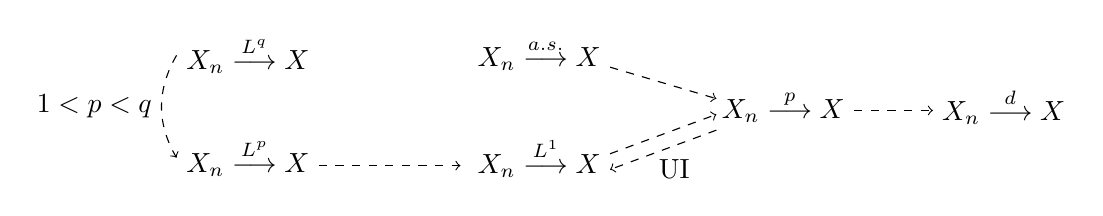
\begin{tikzpicture} 
		\draw (-5.7,1.3) node (Lq) {$X_n\stackrel{L^q}{\longrightarrow}X$} ;
		\draw (-5.7,0) node (Lp) {$X_n\stackrel{L^p}{\longrightarrow}X$} ;
		\draw (-2,0) node (L1) {$X_n\stackrel{L^1}{\longrightarrow}X$} ;
		\draw (-2,1.3) node (as) {$X_n\stackrel{a.s.}{\longrightarrow}X$} ;
		\draw (1.1,0.65) node {$X_n\stackrel{p}{\longrightarrow}X$} ;
		\draw (3.9,0.65) node {$X_n\stackrel{d}{\longrightarrow}X$} ;
		
		\draw[->,dashed] (-1.1,1.15) -- (0.25,0.75) ;
		\draw[->,dashed] (-1.1,0.05) -- (0.25,0.55) ;
		\draw[->,dashed] (0.25,0.35) -- node[below]{\hspace{8pt}UI} (-1.1,-0.15);
		\draw[->,dashed] (2,0.6) -- (3,0.6) ;
		\draw[->,dashed] (-4.8,-0.1) -- (-3,-0.1) ;
		\draw[->,dashed] (Lq.west) to[out=-120,in=120] node[left]{$1<p<q$} (Lp.west);
		\end{tikzpicture}
\end{proposition}

\newpage

\begin{thebibliography}{99}  
	\bibitem{ref1}Athreya, Krishna B., and Soumendra N. Lahiri. \emph{Measure theory and probability theory}. Vol. 19. New York: Springer, 2006.
\end{thebibliography}

\end{document}
